\section{Методы расчета поверхностей в молекулярном моделировании} \label{part1_3_sasa}
\textit{Раздел \ref{part1_3_sasa} изложен согласно кандидатской диссертации автора \cite{shaytan_thesis_kfmn_2010} << }
Поверхность доступная растворителю (ПДР) (solvent accessible surface area (SASA)) -- это поверхность биомолекулы, которая доступна растворителю. Обычно ПДР выражают с квадратных ангстремах. ПДР была впервые описана Ли и Ричардсом\cite{lee_richards} и иногда называется молекулярной поверхностью Ли-Ричардса, она определяется как поверхность которую описывает центр пробной сферы при ``обкатывании'' сферы вокруг молекулы. Размер сферы обычно берётся порядка размера молекулы воды. В этом плане ПДР можно воспринимать, как расширенную поверхность Ван-дер-Ваальса.

Кроме ПДР широкое распространение получила поверхность Коннолли, которая представляет собой как бы полость, которая формируется в растворителе при помещении в него молекулы. Коннолли разработал также полуаналитический метод расчёта такой поверхности \cite{connolly_1983}.

На Рис. \ref{f:2_surf} изображены поверхности доступные растворителю и молекулярные поверхности Коннолли для модельной системы.

\begin{figure}[htbp]
   \centering
   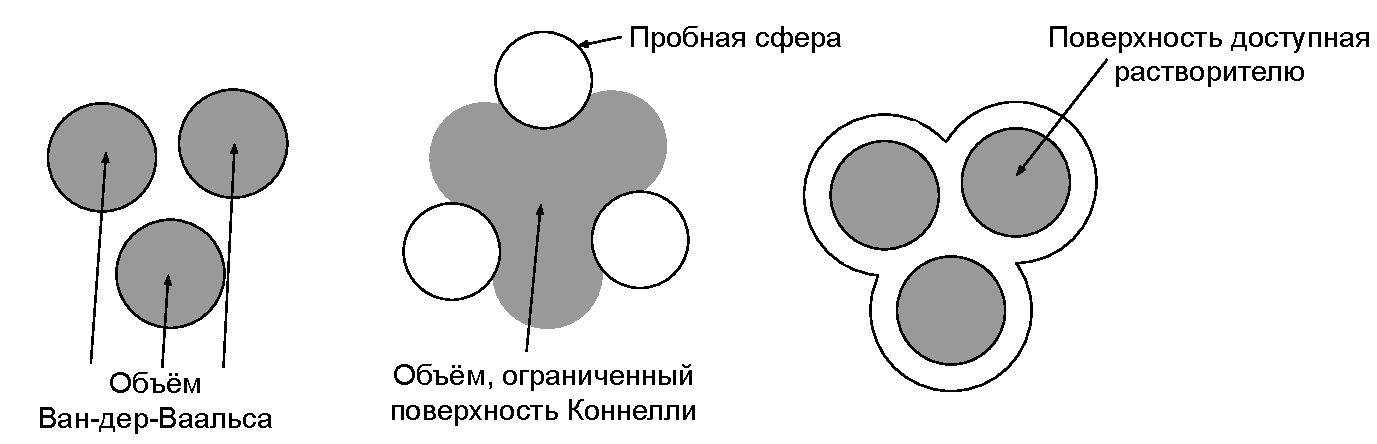
\includegraphics[width=15cm]{images/2_surf}
      \caption{Пояснения к определению поверхности доступной растворителю и поверхности Коннолли.}
   \label{f:2_surf}
\end{figure}
\textit{>>}